\chapter{Courses 2 system}

\label{kap:courses} % id kapitoly pre prikaz ref

\section{Introduction}
% TODO: culik
\paragraph{}
In 2010, a new approach of the learning was implemented in the web design course in our faculty. A blog based learning. This approach is based on blog posts about the lectures content written by the students. These blogs are published and they are rated by the teachers and the students. The ratings of the blog are included in the final subject result. This approach forces the students to study lectures more precisely and they have to read the blog posts of their classmates, which make the students focused on the discussed problems.\cite{culik}

\paragraph{}
Since the blog portal \cite{rejda} was running in the faculty, there was a space to publish the blog posts. Unfortunately, there was not a system to process the reviews and ratings of these posts. The necessity of this system occurred. One possible solution was to integrate mentioned functionality into existing blog portal, other one was to create a separate system with a possible blog integration. For our purpose there was choosen the second solution. The goal of a standalone system development was to create the customizable modular Learning management system. Such system should o er the blog portal integration (and/or provide an API for an integration with the other systems), implement the basic learning management system requirements (course management, user management, content management, etc.) and o er a logical and user friendly structure for the next developers.

% TODO uz je moje
\paragraph{}
The Courses system was developed as the result of the bachelor thesis from 2013 called Integrated learning management system.\cite{culik} Courses was deployed to the production usage in 2013 and 4 courses were running on Courses system for two semesters. The system was used by 130 users in system and 6 teachers. Although the system was designed as a fully modular system with an integration with blog portal, there appeared some flaws during the production usage.

\paragraph{}
Courses 2 is a second iteration of learning management system developed at the Comenius University by Jakub Culik.  This system aims at modularity with easy module management and usability for students and teachers. During its development it has been already used to teach multiple courses and increasingly gained popularity among teachers. After finishing of base development in autumn of 2014 multiple enhancements of this system and particulary assignments module were needed to be implemented.


\subsection{Problems and focus of this work}

\paragraph{}
Full development of this system was finished in the spring of 2015. Since then, various bugs were discovered that needed to be solved. One of the purposes of this work is to provide support for this system and fix these issues.

\paragraph{}
During usage of Courses 2 we descovered that it is important to enable peer review and improved submissions in assignments module. The flow is following: student is assigned an assignment and submits his solution. After that, this solution is peer reviewed and student gets feedback from other students. Then, he is enabled to submit an improved solution of this assignemnt. This work was also published as article "Peer Review Support in a Virtual Learning Environment"  \cite{homola2016peer}.

\paragraph{}
Another extension to Courses 2 system was support for team assignment management. Team assignemnts has appeared to be important in the process of learing. This extension was first used by "Modern approaches to webdesign" course and used by about 50 students. It was also aim of one diploma thesis to develop this extension.

\paragraph{}
Hovewer the most important part of this work was to implement easy to use web mirroring. In some courses, students were submitting URLs of their web projects, not the sources itself. This enabled the students to use technologies which they wanted to use to develop their web pages and teacher reviewed only the rendered page. The problem was that student was able to alter his project anytime he wanted to do, so there were plenty of room for cheating. We needed to develop the technology to auto backup the rendered pages in such cases. In this work, we present simple and elegant solution of this problem.


\paragraph{}
Purpose of this chapter is to provide information about this system as it was implemented, with focus on assignments module so that we could later explain our contribution to this system.
 
\begin{figure}[t]
    \centering
    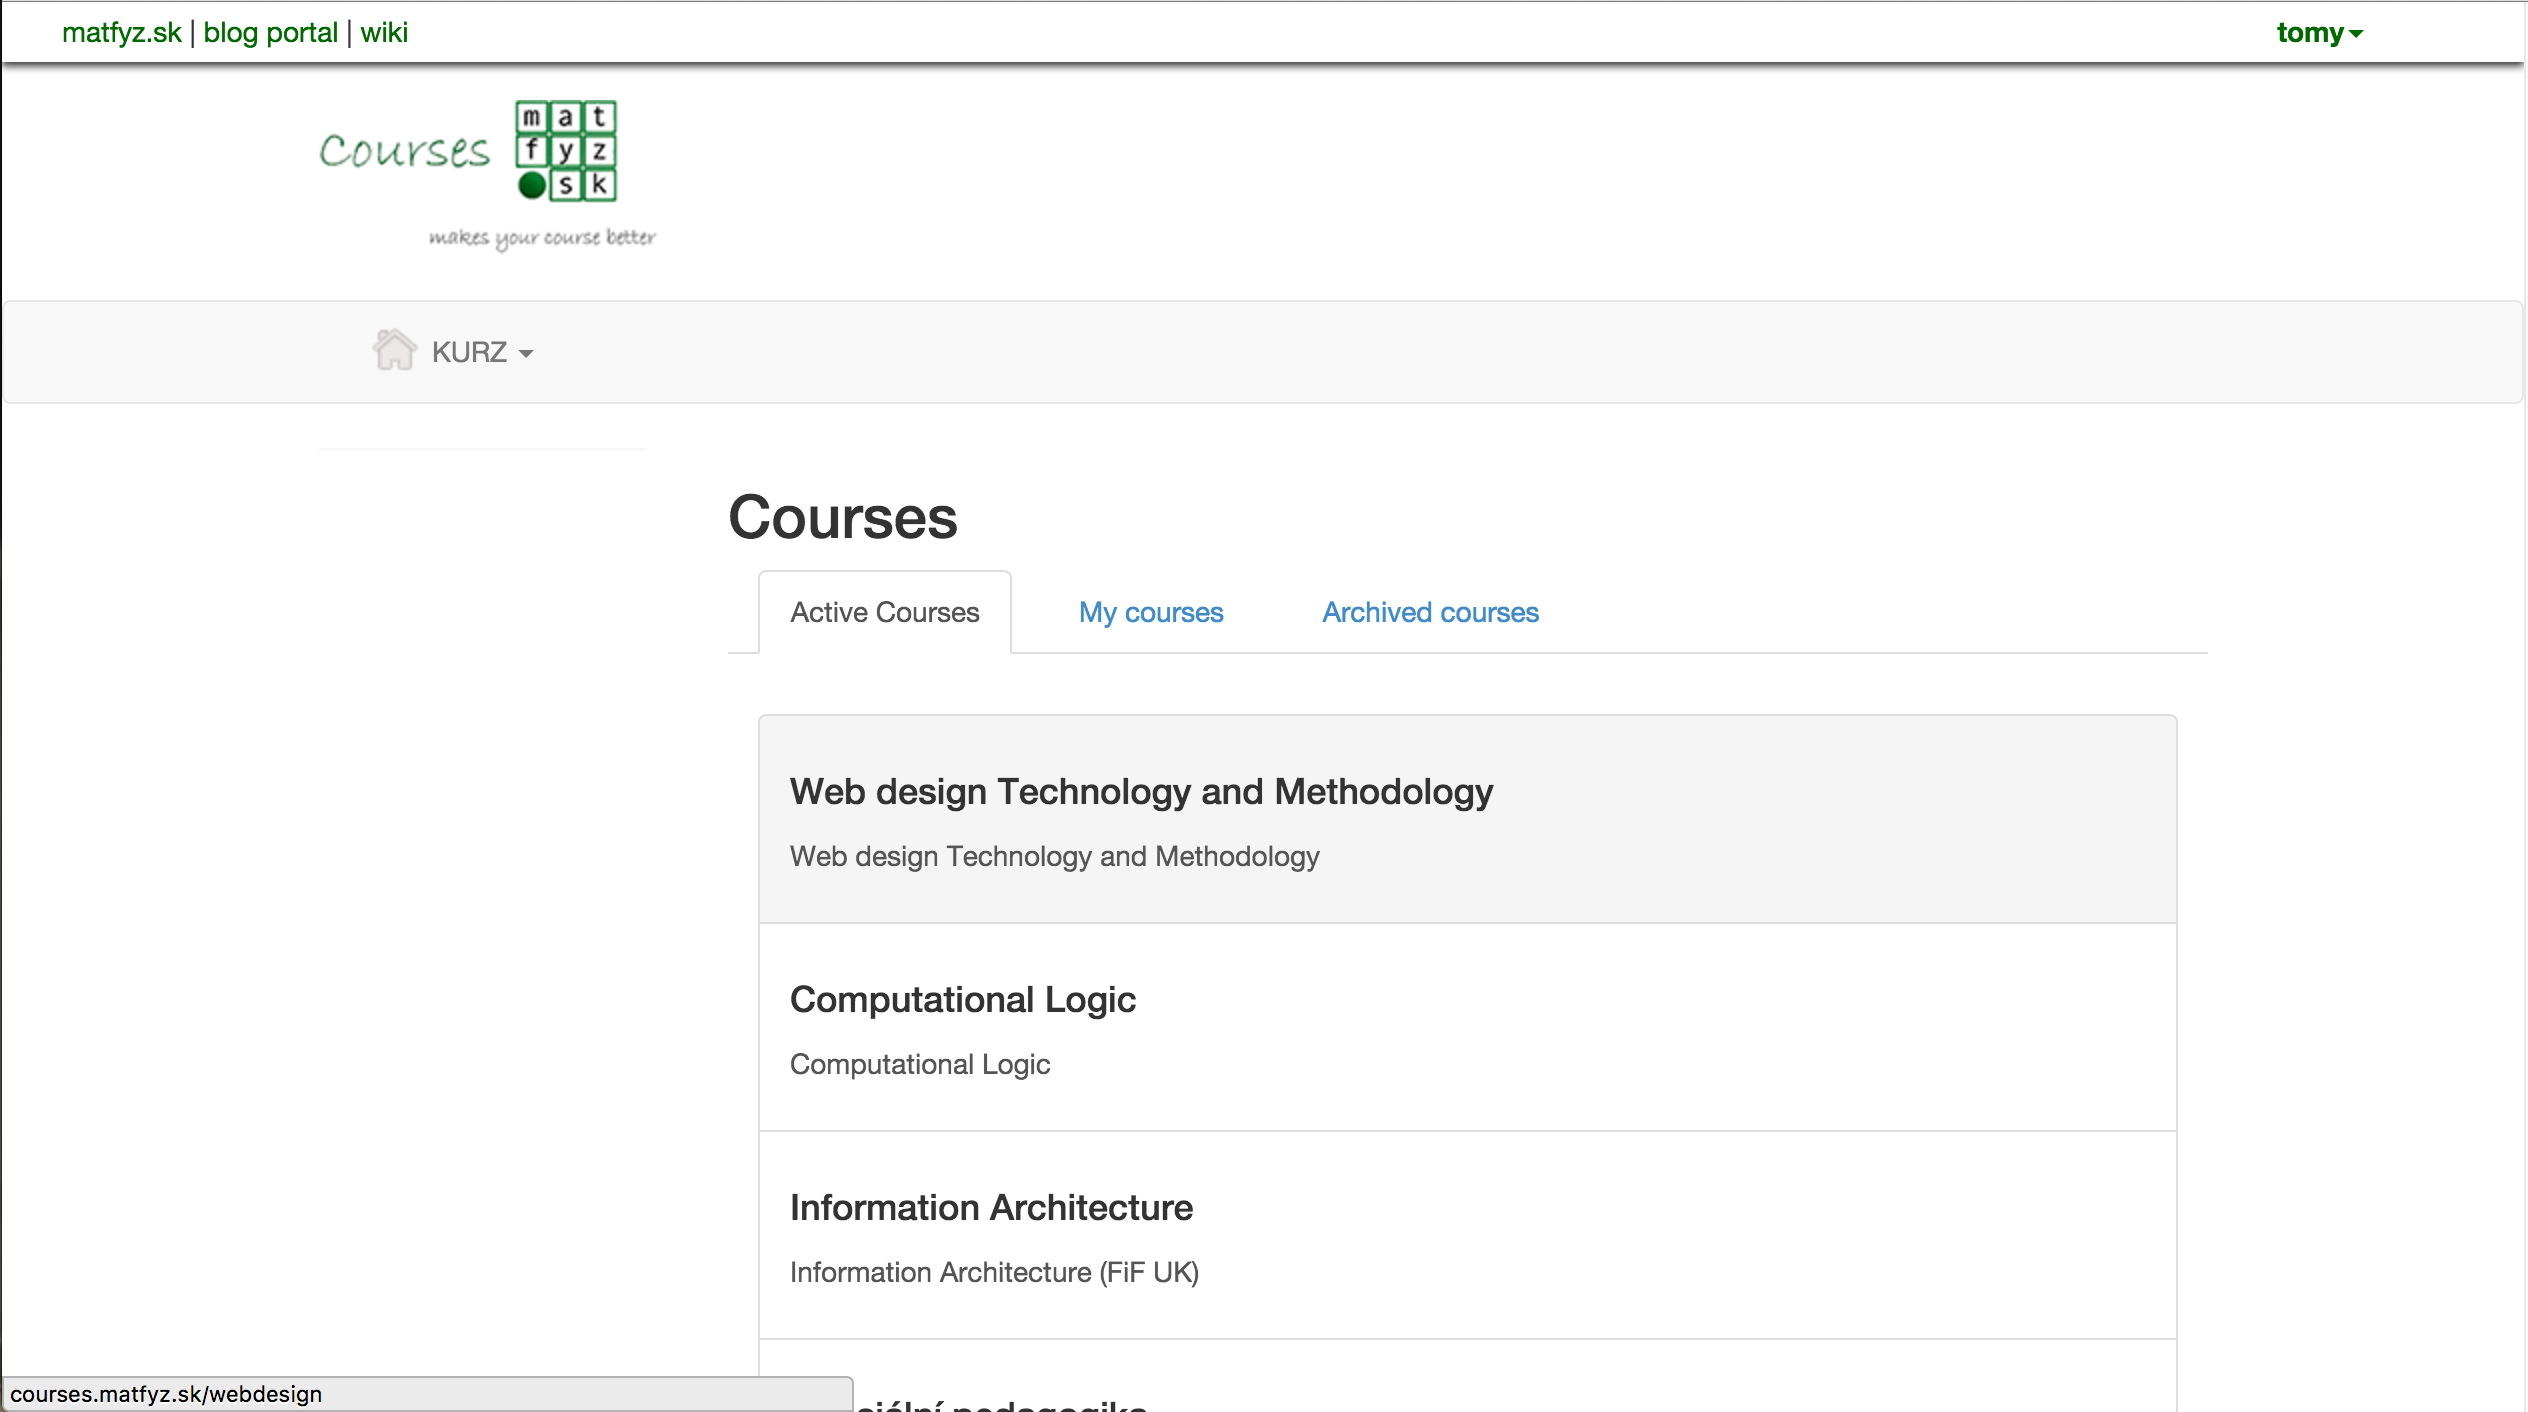
\includegraphics[width=0.9\textwidth]{courses/screenshot.png}
    \caption{Screenshot of Courses 2 main page}
    \label{courses_main}
\end{figure}


\section{Overview}
\paragraph{}
Aim of the Courses 2 system is to provide all functionality splitted into modules. These modules can then be easily extended an improved separately, which helps reduce number of bugs and issues. After finished development of this system, 3 modules were introduced \cite{culik}.

\paragraph{}
Courses 2 base module provide basic functionality in logging of user and basic course selection as in image \ref{courses_main}. Notes module, on the other hand provides functionality of static content, such as lectures, labs, project tasks and information about courses. The role of results module is to provide scores for all students attending a course. The last one, assignments module is the purpose of this work, so it is described in it's own part.

\section{Assignments module}
\paragraph{}
Purpose of the assignments module is to provide student and teacher interface for management, submission and reviewing of assignments. This is the most complex module but we found that is still lacking some functionality and therefore must be extended.

\subsection{Student's part}
\paragraph{}
This module allows students to submit their solutions of assignments and review other students. We found interface of this part counterintuitive so in our future work we decided to refactor it and provide dashboard. This decision was also made after numerous complaints of other students.

\subsection{Teacher's part}


\begin{figure}[h]
    \centering
    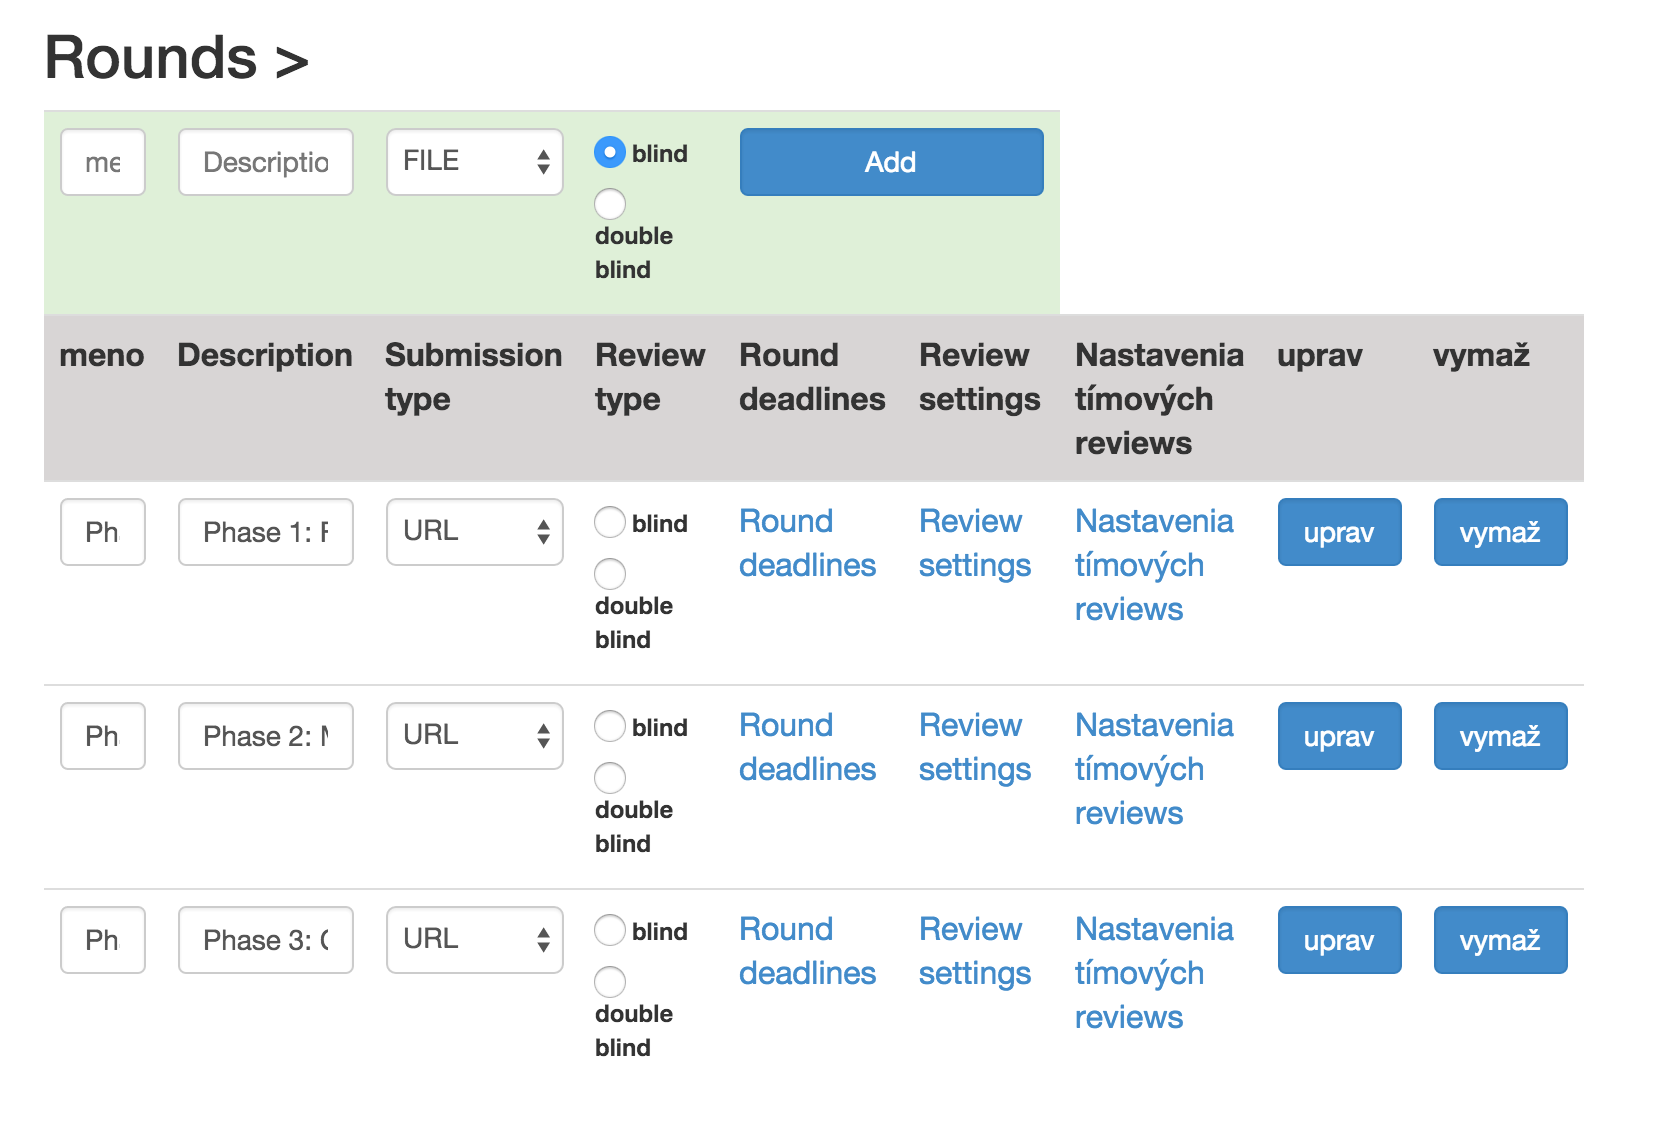
\includegraphics[width=0.9\textwidth]{courses/rounds.png}
    \caption{Assignment management in courses 2 system}
    \label{courses_assignment_admin}
\end{figure}


\paragraph{}
Teacher's part consists of two main functionalities: creating/editing of assignments and evaluating of student submisions. It is also important to note, that assignments module provides also interface for student reviews of other students work as is described in \cite{culik}.

\paragraph{}
Creating and editing of assignments is provided by interface shown on \ref{courses_assignment_admin}. This interface tries to be minimalistic and intuitive but we found that it must be improved. It is important to note that each assignments can have multiple rounds, multiple review settings, notes and can be set to be FILE or URL.

\paragraph{}
The second part of teacher's administration is reviewing of user submissions. Teacher can evaluate a submission after any user submits a submission of assignment and results are than converted into notes module. Along submissions, teacher is also allowed to submit evaluation of student reviews.



\section{Implementation}

\paragraph{}
The whole system is split into modules so it could be easily extended or rewritten. At first we need to describe core of this system, CodeIgniter framework and then we can focus on design patterns and assignments module description.

\subsection{MVC design pattern}
In an Object oriented programming (OOP) programmers often run into problems with application complexity and maintanance of code. As application becomes larger and more robust, it is ofter harder to add or modify existing features. Modifying of complex classes and unclear implementation can cause a lot of software bugs. On the other way, design patterns aim to provide reusable soulutions of common problems in software engineering and reduce this complexity by splitting functionality into specific classes with a single purpose. One of the most important desing patterns is Model
View-Controller, which is the performs as the core of the CodeIgniter framework.

\paragraph{}
Model-View-Controller (MVC) design pattern was first created in 70's by SmallTalk programmers. Since that time, MVC design idiom has become a commonplace, especially in object oriented systems \cite{mvc}. We specify the motto of this pattern as to "Stop data, program logic and presentation layers being mixed up together".

\paragraph{}
To do so, MVC has to split application functionality into three layers: models, views and controllers. Each part plays specific, distinctive, non-overlapping function. This also enables programmers to easily replace these layers and extend functionality. To fully understand this pattern, we need to look at each layer separately with context to CodeIgniter framework.

\subsubsection{Model}
\paragraph{}
Model is basicaly a class where all of the business logic is stored. Basic model operations are create, update, read, delete (often referenced as CRUD) of application data plus handling of external services (such as API calls). In CodeIgniter model is the only MVC layer supposed to perform operations with database. CRUD operations are forbidden outside models to prevent programming bugs and to keep simplicity of the code base.

\paragraph{}
In Courses 2, models are connected to MySQL database which stores all the data about courses, users and teachers. There are also models, which use Oauth2 protocol to communicate with external services to authorize users from other matfyz portals. In this way, there is no more need to store passwords in MySQL database because log in of user is handled outside of application and this improves security.

\begin{lstlisting}
class Admin_model extends MY_Model
{
    function __construct()
    {
        parent::__construct();
    }

    public function get_assignment($id)
    {
        $where = array (
            'course_id' => $this->cid,
            'id' => $id,
        );
        return $this->db->get_where('assignment', $where)->row_array();
    }

    public function add_assignment($name)
    {
        $input = array (
            'name'      => $name,
            'course_id' => $this->cid
        );
        return $this->db->insert('assignment', $input);
    }

    public function update_assignment($id, $name)
    {
        $where = array (
            'id'        => $id,
            'course_id' => $this->cid
        );
        $update = array (
            'name'      => $name,
            'course_id' => $this->cid
        );
        return $this->db->where($where)->update('assignment', $update);
    }
    
    .... (another 200 lines of code)
\end{lstlisting}

\paragraph{}
Example above presents a model of assignment in Courses application. This model is used by all of the controllers and serves as the only code accessing or editing assignment in database.

\subsubsection{View}
Views, unlike controllers and models are not supposed to contain any logic. In object-oriented terms, these will consist of sets of classes which give us "windows (such as GUI, CLI or API) \cite{mvc}. Althought views are very often graphical, they don't have to be. Example of view from Courses application could be something like this:

\begin{lstlisting}
<h3>Assignments</h3>

<?php foreach ($assignments as $assignment) : ?>
    <div class="alert alert-info">
        <a href="<?= $course->course_base() ?>assignments/<?= $assignment['id'] ?>">
            <?= $assignment['name'] ?>
        </a>
    </div>
<?php endforeach; ?>

<?php if (!$assignments) : ?>
    <div class="alert alert-warning">
        <?= lang('assignments_found') ?>
    </div>
<?php endif; ?>
\end{lstlisting}

\subsubsection{Controller}
A controller is an object that manipulates a view \cite{mvc}. Over-simplifying a bit, controller knows all the enviroment settings (operating system, display resolution, ...) and according to these loads data from models, perform operations on them and then they are sended to a view. Controller knows the views but views does not. The same applies to models. Example of controller connecting previous model with view could be:

\begin{lstlisting}
    public function run()
    {
        $assignments = $this->assignments_model->get_course_assignments();

        for ($i=0; $i<count($assignments); $i++) {
            $notes = $this->assignment_note_model->get_assigment_notes($assignments[$i]['id']);
            $assignments[$i]['notes'] = $notes;
        }

        $data = array (
            'assignments' => $assignments,
        );

        $this->layout->set_content('../modules/assignments/views/user/assignments', $data);
    }
\end{lstlisting}

\paragraph{}
As we can see, in controller, data are loaded from models, then this layer can perform some operations over them and after all, result is sent to model which is then rendered.


\begin{figure}[h]
    \centering
    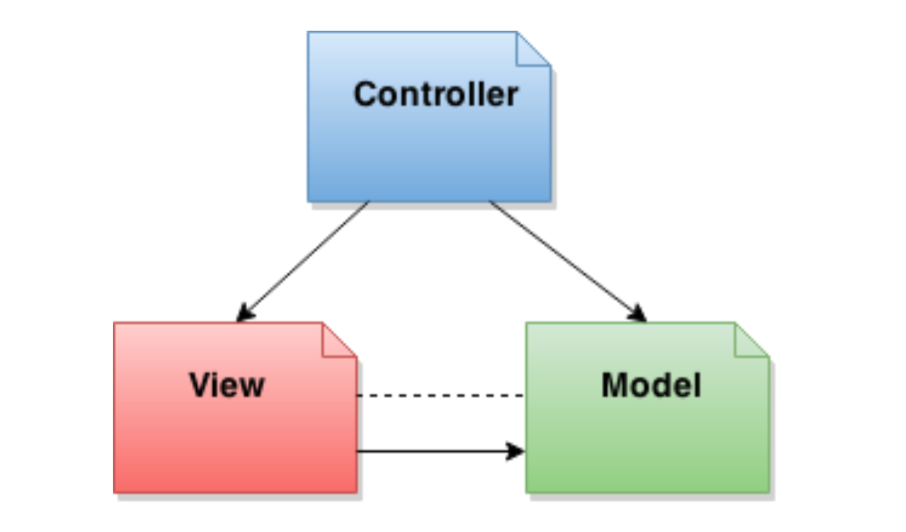
\includegraphics[width=0.6\textwidth]{courses/mvc.png}
    \caption{MVC pattern data flow}
    \label{mvc_data_flow}
\end{figure}

\subsubsection{MVC summary}
\paragraph{}
Although MVC was originaly developed for desktop computing \cite{mvc} it is mostly used to build web applications. This fact is reflected in most frameworks and in CodeIgniter too. Splitting the application in three separate layers can bring simplicity, code reusability and easily switchable GUIs.

\section{HMVC design pattern}
\paragraph{}
Using MVC design pattern is excellent for building small applications. Hovewer, huge application building on pure MVC pattern brings also some disadvantages \cite{culik}. For example, large sets of views, models and controllers could be a point of confusion and failure for many programmers. In case of larger projects, it is very needed to bring order to MVC. Solution to this can be Hierarchical Model-View-Controller design pattern (HMVC) \cite{hmvc}.

\paragraph{}
Hierarchical Model-View-Controller design pattern (HMVC) is a direct extension of the MVC pattern that aims to solve mainly scalability issues mensioned earlier. HMVC was first described in a blog post entitled HMVC: The layered pattern for developing strong client tiers on the JavaWorld web site in July 2000 \cite{hmvc}. In summary, HMVC is a collection of MVC triads operating as one application. Each of this triads is treated as individual and can be rendered on it's own. This resolves into greater scalability, code reusability and most importantly, resolves the problem with hudge views in large projects.

\begin{figure}[h]
    \centering
    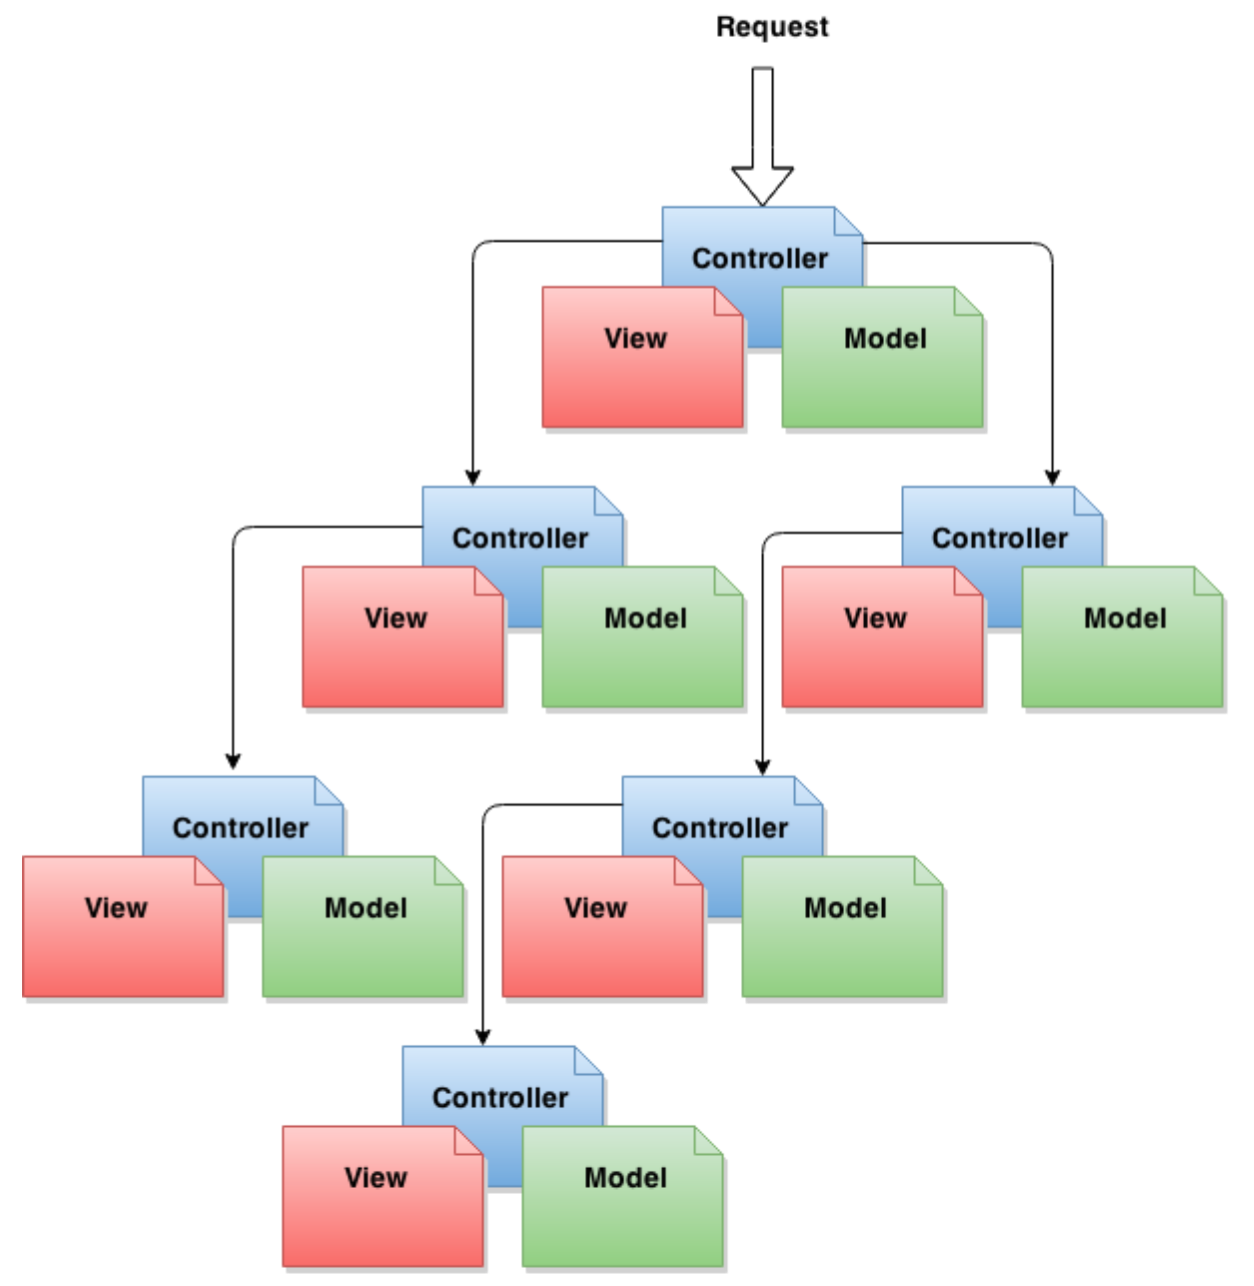
\includegraphics[width=0.7\textwidth]{courses/hmvc.png}
    \caption{Scheme of HMVC design pattern}
    \label{fig:awesome_image}
\end{figure}


\paragraph{}
To successfuly implement HMVC, it is crucial for application to be broken into systems \cite{hmvc}. Each system gets it's own views, models and controllers and is fully in control of it's own part and nothing else. In Courses 2 system, these systems are called modules (assignments, note, quiz, ..). Thanks to HMVC model, in our further work, we will only edit assignments module and can ommit descriptions and refactoring of other modules.

\paragraph{}
We also must note, that CodeIgniter framework, core of the Course 2 system is not directly supporting HMVC design pattern. This improvement was implemented thanks to Jakub Culik \cite{culik}.


\subsection{CodeIgniter framework}
\paragraph{}
CodeIgniter is an Application Development Framework - a toolkit - for people who build web sites using PHP  \cite{codeigniter}. One of it's goals is to provide exceptional performance of web applications along with minimum complexity and fast development. CodeIgniter was born from ExpressionEngine \cite{elislab} in 2006 and since then, it increasingly gained popularity among PHP developers. In 2008 CodeIginiter became industry leader in an enviroment saturated with PHP frameworks \cite{elislab} and in 2014 CodeIgniter v 2.2 was released.

\paragraph{}
This framework is licensed under custom Elislab license, which is basicaly an open source license with only a few restrictions \cite{elislablicense}. We provide a copy of this license in medium attached to this work.


\begin{figure}[h]
    \centering
    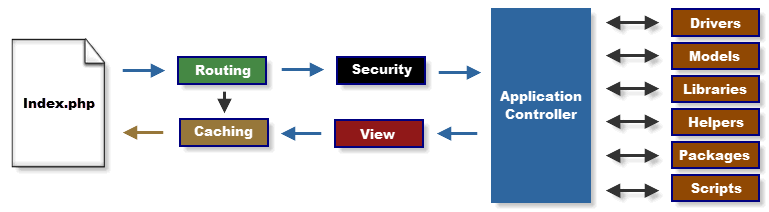
\includegraphics[width=0.85\textwidth]{courses/codeigniter.png}
    \caption{CodeIgniter request flow}
    \label{codeigniter_flow}
\end{figure}

\paragraph{}
To understand how CodeIgniter works, let's look at processing of HTTP requests in this framework. CodeIgniter uses Apache2  module \texttt{mod rewrite}. This allows to be firstly processed \texttt{index.php} file as seen on image \ref{codeigniter_flow}. Purpose of this script is to load configuration of whole application, load routes, cache and other classes. It is provided by CodeIgniter framework and should not be changed (only for configuration purposes).

\paragraph{}
To process HTTP request, router must decide correct operation over it. If a cache file exists, it is sent directly to the browser, bypassing the normal system execution \cite{codeigniter}. Before the application controller is loaded, the HTTP request and any user submitted data is filtered for security.

\paragraph{}
In the next step, routing takes place. Each module of application must have it's own routes defined as follows:

\begin{lstlisting}[basicstyle=\small]
$route[course/(:num)'] = "courses/$1";
\end{lstlisting}


\paragraph{}
The application takes list of all routes and applies the one of which regexp pattern matches the request URL. After this operation, proper controller (that must extend \texttt{CI\_ CONTROLLER} class) is selected, instanciated and method \texttt{run()} of this controller is run.

\paragraph{}
This controller loads data from models, can perform some operations over them and then data are sent directly to view. The finalized View is rendered then sent to the web browser to be seen. If caching is enabled, the view is cached first so that on subsequent requests it can be served.

\paragraph{}
Since our modification of CodeIgniter uses HMVC desing patter, there is a slight change in usual data flow. Selected controller can run one, or more controllers that renders their own response parts which are then send to his view as basic string and rendered there.

\section{Comparision of other learning management systems}
\paragraph{}
In this section, we consider important to describe alternative learning management systems to Courses 2. Although many projects exists, none of them met our criterions and considerations. This section is important to realize why we had to write our own learning management system that is easily extendable and usable.

\subsection{Moodle}
\paragraph{}
Moodle is a free, online Learning Management system enabling educators to create their own private website filled with dynamic courses that extend learning, any time, anywhere \cite{moodlesite}. This system is trying to deliver full palette of functionalities, tools, modules, language support with focus on security and usability. It was developped by its Lead Developer Martin Dougiamas in 1999 with first public release in 2002. Since than moodle quickly gained popularity among famous universities like Oxford (2004) and became leading and award-winning open source LMS in 2007. \cite{moodlesite}

% TODO: Delete
\paragraph{}
Moodle as a learning platform can enhance existing learning environments. As an E-learning tool, Moodle has a wide range of standard and innovative features such as calendar and Gradebook. Moodle is a leading virtual learning environment and can be used in many types of environments such as education, training and development and in business settings \cite{moodlesite}



\paragraph{}
Hovewer, there are few considerations to make. Over the time, Moodle has grown to be huge piece of software with hundreds of thousands lines of code and large number of extensions. Other side of this is that this makes future development very hard and time-consuming. The next disadvantage is that new pieces of code are hardly maintained and require skilled developers.

\paragraph{}
The next thing Moodle is currently not supporting are assignment rounds, assignment reviews and team assignments. There may be some plugins for this functionality but we do not consider them useful or maintained. We also found that writing plugins for moodle is not an easy task. Hovewer, on the end of this work we are going to present a Moodle plugin for mirroring URLs and saving mirrored files as user's submission.

\begin{figure}[t]
    \centering
    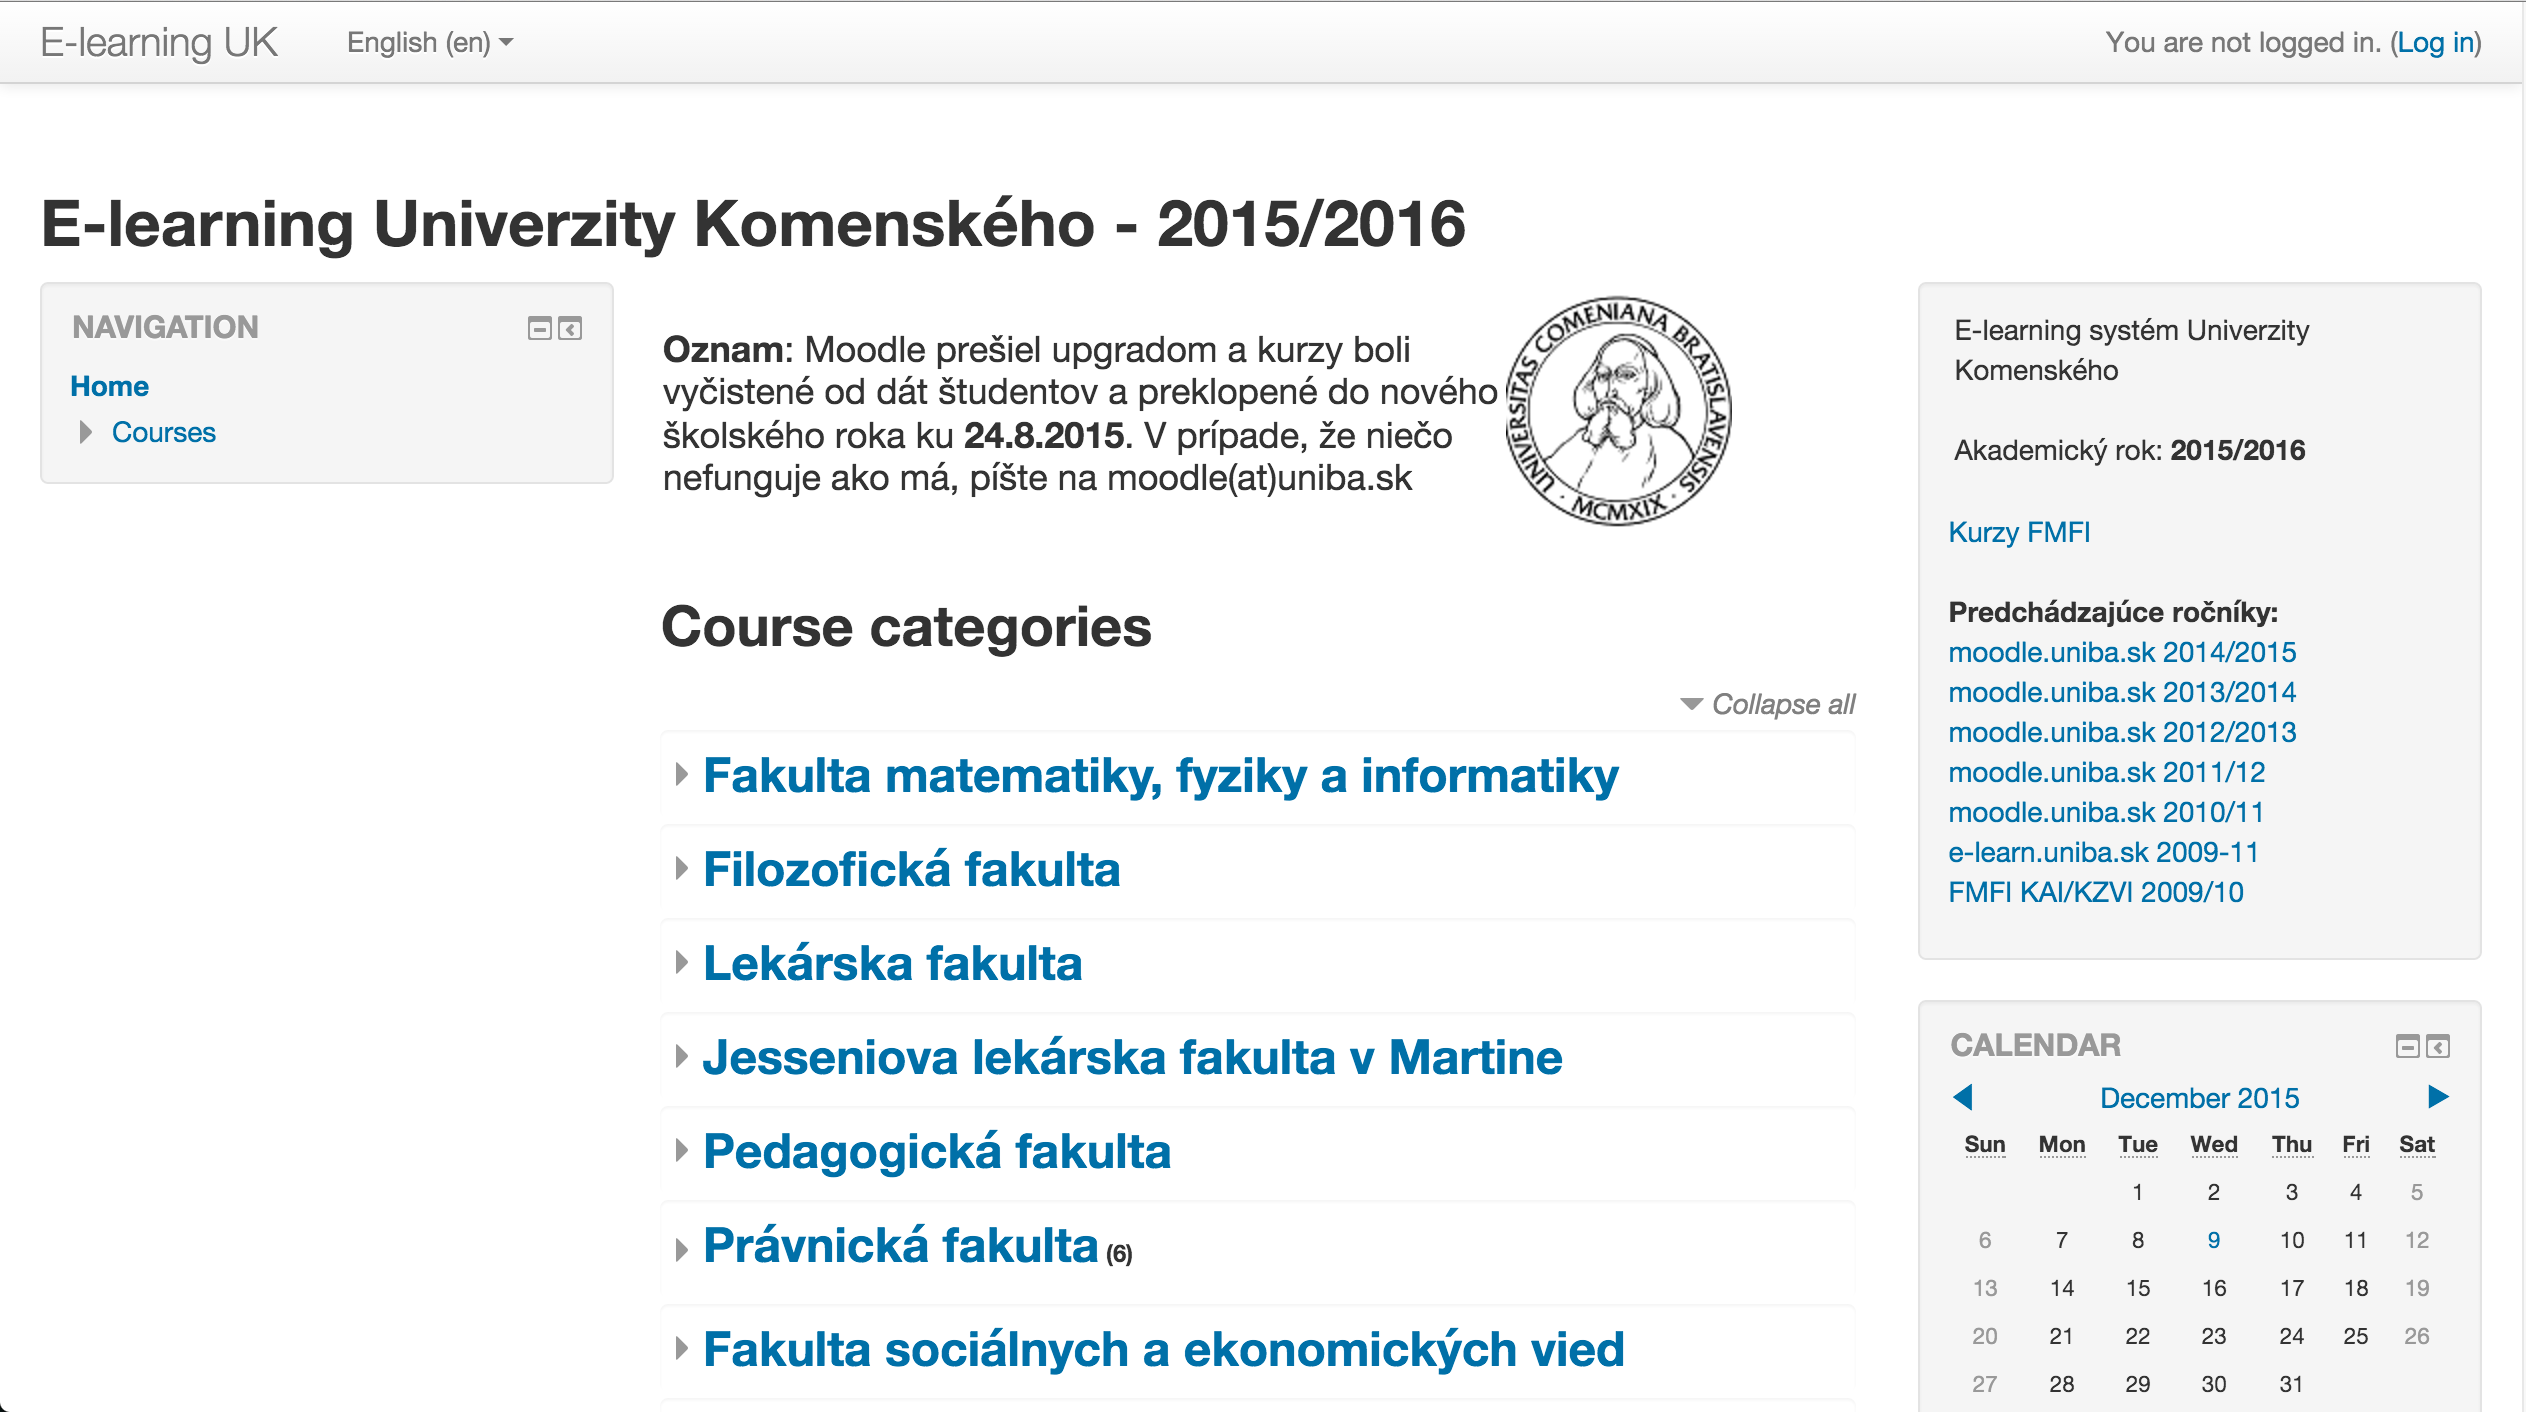
\includegraphics[width=\textwidth]{courses/moodle.png}
    \caption{Screenshot of Comenius University Moodle}
    \label{moodle_pic}
\end{figure}

\subsubsection{Moodle Workshop}
\paragraph{}
Workshop is a peer assessment activity with many options. Students submit their work via an on line text tool and attachments. There are two grades for a student: their own work and their peer assessments of other students' work
\cite{moodleworkshop}. This plugin is avaible on official Moodle site and can work with many versions of Moodle. 

\paragraph{}
We found, that this plugin aims to support same functionality as we in Moodle. We appreciate this opportunity but does not consider it sufficient for our purposes.

\begin{figure}[t]
    \centering
    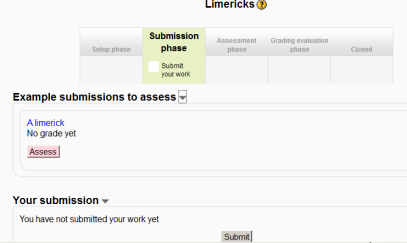
\includegraphics[width=0.7\textwidth]{courses/moodleworkshop.png}
    \caption{Moodle workshop plugin}
    \label{moodle_workshop}
\end{figure}

\subsection{Blackboard}
\paragraph{}
Blackboard Learn (previously the Blackboard Learning Management System), is a virtual learning environment and course management system developed by Blackboard Inc. It is Web-based server software which features course management, customizable open architecture, and scalable design that allows integration with student information systems and authentication protocols. It may be installed on local servers or hosted by Blackboard ASP Solutions. Its main purposes are to add online elements to courses traditionally delivered face-to-face and to develop completely online courses with few or no face-to-face meetings. \cite{blackboard}

\paragraph{}
According to research, Blackboard received 41 percent market share as of fall 2013 among other learning management system. This makes Blackboard the most used tool in industry

\paragraph{}
Hovewer, Blackboard brings many disadvantages. Mainly, Blackboard is not avaible as open source software and is sold under custom license. Other issues with Blackboard LMS are several legal issues, including faulty patent rights claims. We consider this facts to be enough to not use Blackboard.

\subsection{Desire2Learn}
\paragraph{}
Desire2Learn was founded in 1999 by president and CEO John Baker \cite{d2l}. This LMS aims to be online teaching and learning platform that’s easy, flexible, and smart. This technology is used by more than 1,100 clients and 15 million learners in higher education, K–12, healthcare, government, and the enterprise sector.

\begin{figure}[h]
    \centering
    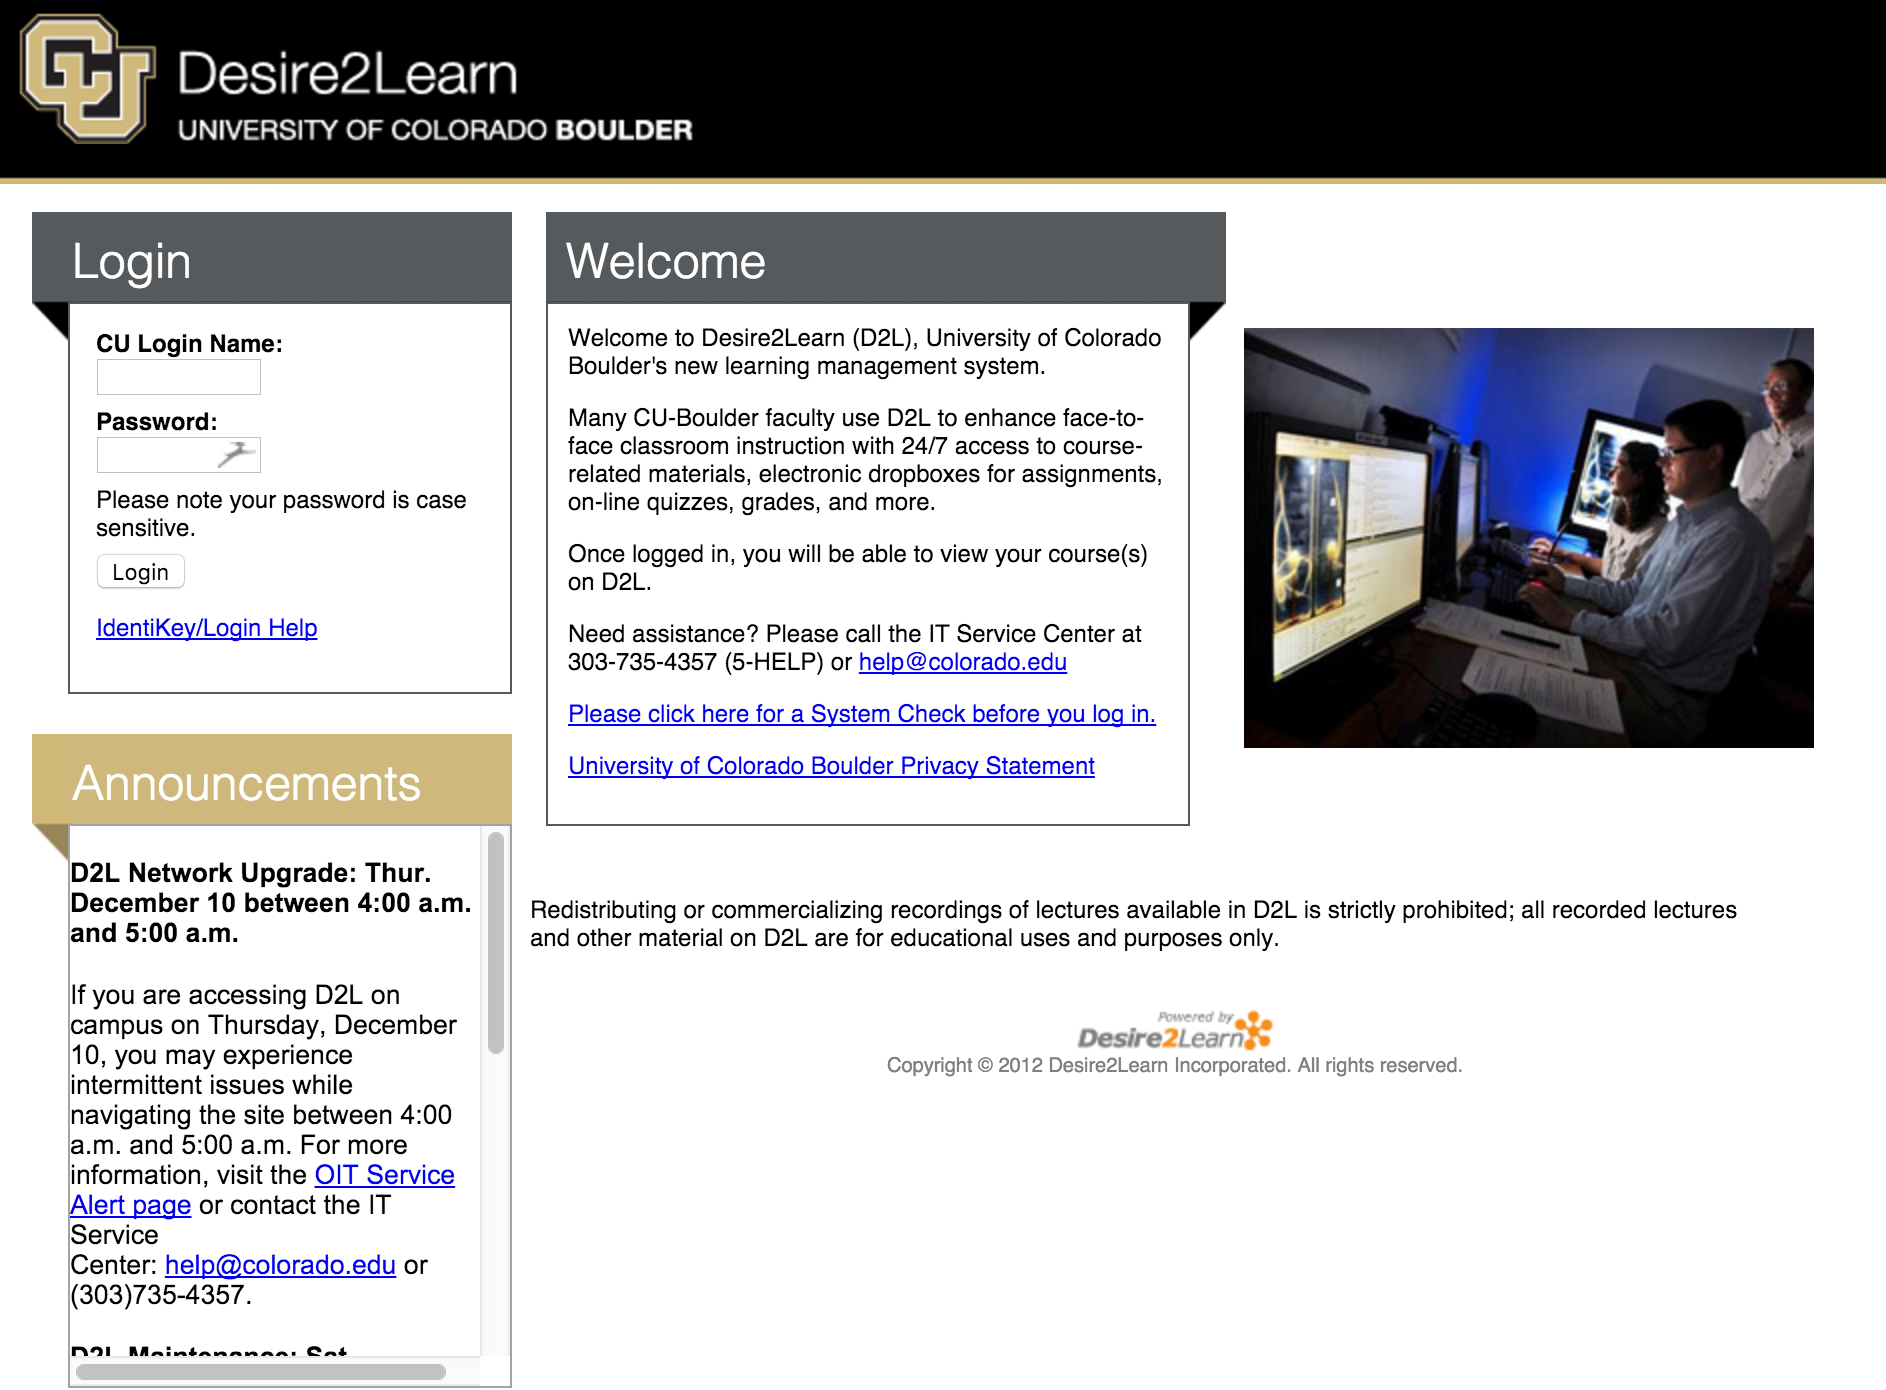
\includegraphics[width=\textwidth]{courses/d2l.png}
    \caption{Desire2Learn Screenshot}
    \label{d2l}
\end{figure}

\paragraph{}
Hovewer, Desire2Learn is not an option for our purposes. This system is commercial and not open source so it is imposible to use it for our future work.

\subsection{Conclusion}

\paragraph{}
We presented multiple alternative learning management systems. All of them were robust, secure and maintained systems hovewer the complexicity was fairly great so we consider developing our own LMS to be the best option. The next important fact in our decision process was that many of these LMS are not licensed under an open source license.

\paragraph{}
In the next part of this work, we are going to focuse on modifications and improvements with assignment module, mainly team assignments, mirroring of assignment submissions, assignment dashboard and peer review and improved submissions in assignments.